\documentclass[runningheads]{llncs}
\usepackage[ruled]{algorithm2e}
\usepackage{amsfonts}
\usepackage{amsmath}
\usepackage{bm}
\usepackage{booktabs}
\usepackage{color}
\usepackage[compress]{cite}
\usepackage{graphicx}
\usepackage{hyperref}
\usepackage{physics}

\renewcommand\UrlFont{\color{blue}\rmfamily}
\SetKwInput{KwHyperparameters}{Hyperparameters}
\SetKwInput{KwInput}{Input}
\SetKwInput{KwOutput}{Output}
\SetKwComment{Comment}{/* }{ */}
\DeclareMathOperator{\sgn}{sgn}
\DeclareMathOperator*{\argmax}{arg\,max}

\begin{document}

\title{
  A Branch-and-Bound Algorithm for the Ticket Restaurant Assignment Problem
}
\author{Gabriele Cerizza}
\authorrunning{G. Cerizza}

\institute{Università degli Studi di Milano\\
\email{gabriele.cerizza@studenti.unimi.it}\\
\url{https://github.com/gabrielecerizza/orc_project}}

\maketitle

\section*{Introduction}
\label{sec:introduction}

In this report we detail a branch-and-bound exact method based on Lagrangean relaxation to solve the ticket restaurant assignment problem (TRAP), pursuant to the project specifications set out for the Operational Research Complements course of the Università degli Studi di Milano\footnote{\url{https://homes.di.unimi.it/righini/Didattica/ComplementiRicercaOperativa/ComplementiRicercaOperativa.htm}}. 

In Section~\ref{sec:dataset} we illustrate the dataset used in the experiments. In Section~\ref{sec:algorithm} we briefly describe the algorithm and its implementation. In Section~\ref{sec:experiments} we show the results of our experiments and provide comments on them. Finally, Section~\ref{sec:conclusions} contains our concluding remarks. 

\section{Ticket Restaurant Assignment Problem}
\label{sec:problem}

In this section we define the TRAP (Section~\ref{subsec:problem:definition}), we formalize it as a mathematical programming problem (Section~\ref{subsec:problem:formalization}) and we examine the relevant literature (Section~\ref{subsec:problem:related_works}).

\subsection{Definition}
\label{subsec:problem:definition}

The TRAP is defined as follows. A ticket company (TC) possesses two kinds of restaurant tickets: the low-profit tickets and the high-profit tickets. TC gives a certain amount of tickets to customer companies (CC). Each CC receives only one kind of tickets. Each CC has different sets of employees and each set uses the tickets to buy meals in a specific restaurant.  

For each restaurant with which TC has a deal, a given ratio between low-profit and high-profit tickets must be observed. 
The TC must maximize the profit while complying with this constraint. Thus, maximizing the profit amounts to minimizing the number of low-profit tickets while ensuring that a given amount of low-profit tickets is assigned for each considered restaurant.

\subsection{Formalization}
\label{subsec:problem:formalization}

Let $I = \{1,\dots,m\}$ be a set of restaurants, $J = \{1,\dots,n\}$ be a set of customer companies, $b \in \mathbb{Z}_{+}^{m}$ be the vector representing the minimum amount of low-profit tickets to be assigned for each restaurant, and $A \in \mathbb{Z}_{+}^{m \times n}$ be the matrix representing the amount of low-profit tickets assigned to each given customer company for each given restaurant, so that $a_{ij}$ is the amount of low-profit tickets assigned to customer company $j$ for restaurant $i$. Then, the integer linear programming model of the ticket restaurant assignment problem is the following:
\begin{alignat}{3}
  &\min & \quad & z = \sum_{j \in J} \left( \sum_{i \in I} a_{ij} \right) x_j \label{eq:primal}\\
  &\text{subject to}  &       & \sum_{j \in J} a_{ij} x_j \ge b_i & \qquad & i = 1,\dots,m \, , \notag\\
  &                   &       & x_j \in \{0,1\}  &\qquad& j = 1,\dots,n \, , \notag
\end{alignat}
where each binary variable $x_j$ indicates whether customer company $j$ is assigned low-profit tickets. We define a cover a vector $x$ such that $Ax \ge b$.

From (\ref{eq:primal}), the following Lagrangean relaxation (LR) is obtained:
\begin{alignat}{3}
  &\min & \quad & z_{\text{LR}} = \sum_{j \in J} \left( \sum_{i \in I} (1 - \lambda_i) a_{ij} \right) x_j + \sum_{i \in I} \lambda_i b_i \label{eq:lagrangean}\\
  &\text{subject to}  &       & x_j \in \{0,1\} & \qquad & j = 1,\dots,n \, , \notag\\
  &                   &       & \lambda_i \ge 0  & \qquad & i = 1,\dots,m \, , \notag
\end{alignat}
where $\lambda_i$ are the Lagrangean multipliers.

Finally, the dual of the linear programming (LP) relaxation of (\ref{eq:primal}) is:
\begin{alignat}{3}
  &\max & \quad & w = \sum_{i \in I} b_i y_i \label{eq:dual}\\
  &\text{subject to}  &       & \sum_{i \in I} a_{ij} y_i \le c_j & \qquad & j = 1,\dots,n \, , \notag\\
  &                   &       & y_i \ge 0  &\qquad& i = 1,\dots,m \, , \notag
\end{alignat}
where $c_j = \sum_{i \in I} a_{ij}$ for all $j \in J$. The dual of the LP relaxation may be exploited to find optimal Lagrangean multipliers (see Section~\ref{subsec:branch-bound:lb}).

The TRAP is a generalization of the set covering problem (SCP), as explained in the following section. The SCP is NP-hard~\cite{caprara-2000-algorithms}, hence so is the TRAP.

\subsection{Related Works}
\label{subsec:problem:related_works}

The problem at hand is equivalent to the SCP when $A$ is a binary matrix and $b$ is an all-ones vector. The SCP has been treated extensively in literature and many of the ideas developed within that context can be leveraged to solve the TRAP. For the SCP, both exact and heuristic algorithms have been devised (see the survey in~\cite{caprara-2000-algorithms}). We focus only on exact algorithms for our problem. 

% However, we stress that large-scale problem instances involving millions of variables and thousands of constraints may be tackled only by heuristic approaches, as observed in~\cite{ceria-1998-lagrangian,caprara-1999-lagrangian}.

The following works in the field of SCP are of particular interest to us. Balas and Ho~\cite{balas-ho-2009-set-covering} adopted a branch-and-cut procedure, comprising a primal heuristic to find upper bounds and subgradient optimization to find lower bounds.
Beasley~\cite{beasley-1987-algorithm} adopted a branch-and-bound procedure, computing upper bounds with a greedy heuristic, computing lower bounds with dual ascent and subgradient optimization, and devising a number of problem reduction techniques.
Balas and Carrera~\cite{balas-carrera-1996-dynamic} adopted a dynamic subgradient-based branch-and-bound procedure to solve the SCP, additionally employing variable fixing techniques and heuristics to obtain upper bounds.

We fashioned our branch-and-bound procedure over the algorithms described in these works, adapting their solutions to account for the peculiarities of the TRAP. In particular, we note that most of the preprocessing techniques exploited for the SCP are unsuited for the TRAP.

A problem more closely related to the TRAP is the one called multicovering problem (MCP)~\cite{hall-hochbaum-1986-fast-approximation, hall-hochbaum-1992-multicovering}, defined as follows:
\begin{alignat}{3}
  &\min & \quad & z = c^\top x \notag\\
  &\text{subject to}  &       & Ax \ge b \, , \notag\\
  &                   &       & x_j \in \{0, 1\}  & \qquad & \forall j=1,\dots,n \, , \notag
\end{alignat}
where $A$ is a binary matrix and $b$ is a vector of positive integers. This problem differs from the one at hand in that $A$ is binary and not simply non-negative.

Notably, Hall and Hochbaum~\cite{hall-hochbaum-1992-multicovering} adopted a branch-and-cut procedure to solve the MCP, using a primal heuristic to find upper bounds and combining a dual heuristic with subgradient optimization to find lower bounds. From this work we derived the main primal heuristic for our branch-and-bound algorithm (see Sections~\ref{subsec:branch-bound:primal} and~\ref{subsec:results:comparisons}). 

Furthermore, a generalization of the TRAP may be identified in the so-called covering integer problem (CIP)~\cite{kolliopoulos-2003-approximating,kolliopoulos-2005-approximation}, defined as follows:
\begin{alignat}{3}
  &\min & \quad & z = c^\top x \notag\\
  &\text{subject to}  &       & Ax \ge b \, , \notag\\
  &                   &       & x_j \le d_j & \qquad & \forall j=1,\dots,n \, , \notag\\
  &                   &       & x_j \in \mathbb{Z}_{+}  & \qquad &  \forall j=1,\dots,n \, , \notag
\end{alignat}
where all the entries in $A$, $b$, $c$ and $d$ are non-negative. This problem is equivalent to the TRAP when the multiplicity constraints $x_j \le d_j$ force $x$ to be binary. Unfortunately, we found only approximation algorithms for the CIP (see~\cite{kolliopoulos-2003-approximating,kolliopoulos-2005-approximation}).

\section{Branch-and-Bound}
\label{sec:branch-bound}

In this section we describe the different aspects of the branch-and-bound algorithm we experimented upon to solve the TRAP: the primal heuristics used to find upper bounds (Section~\ref{subsec:branch-bound:primal}); the techniques used to find lower bounds (Section~\ref{subsec:branch-bound:lb}); the branching rules (Section~\ref{subsec:branch-bound:branch}); and the variable fixing strategies (Section~\ref{subsec:branch-bound:reduction}). 

\subsection{Primal Heuristics}
\label{subsec:branch-bound:primal}

\subsubsection{Greedy heuristic.} This method selects greedily the variables of the cover, picking the row $i$ with the largest ratio between the sum $\sum_{j \in J} a_{ij}$ and $b_i$ and then picking the column with the largest coefficient. Each time a variable is selected, the coefficients on the left-hand side (LHS) and right-hand side (RHS) are decreased accordingly.

In this way we select the row which is easiest to cover, since a larger ratio means that more solutions might satisfy the constraint. Indeed, when the sum $\sum_{j \in J} a_{ij}$ is equal to $b_i$, we must select all variables with non-zero entries in $A_i$ in order to satisfy the constraint, thus restricting the number of possible solutions. By picking the column with the largest coefficient we aim to satisfy the covering constraint in the fastest way.

\subsubsection{Dobson heuristic.} This heuristic is taken from Dobson~\cite{dobson-1982-worst-case} and generalizes an heuristic for the SCP from Chvatal~\cite{chvatal-1979-greedy}. This heuristic picks the column $j$ that minimizes $c_j \sum_{i=1,\dots,m} a_{ij}$. Furthermore, any $a_{ij}$ larger than $b_i$ is lowered down to $b_i$.

The idea of this method is to pick the column that covers the most while costing the least. In the case of the TRAP, however, the cost of each column is equal to the sum of the coefficients of that column, which means that all columns could be equivalently selected. The only exception to this occurs when a column $j$ is enough to cover the remaining part of $b_i$ for any $i$. In this case, $a_{ij}$ would be lowered and therefore $c_j \sum_{i=1,\dots,m} a_{ij}$ would also be lowered. 

In short, this method, applied to the TRAP, prioritizes the columns whose coefficients are enough to cover the remaining part of $b_i$ for any $i$. 

\subsubsection{Hall-Hochbaum heuristic.} This method is adapted from one of the heuristics conceived by Hall and Hochbaum~\cite{hall-hochbaum-1992-multicovering}. Specifically, this method picks the column $j$ that maximizes $\frac{1}{c_j} \sum_{i \in L} \frac{b_i a_{ij}}{\text{space}(i)}$, where $L = \{i \in I : b_i > 0 \}$ and $\text{space}(i) = \sum_{j \in J} a_{ij} - b_i$.

\subsection{Lower Bounds}
\label{subsec:branch-bound:lb}

\subsubsection{Lagrangean relaxation.} A lower bound to the optimal value of problem~(\ref{eq:primal}) can be obtained by solving the LR defined in~(\ref{eq:lagrangean}). When the Lagrangean multipliers $\lambda$ are given, the objective function of~(\ref{eq:lagrangean}) is trivially minimized by setting $x_j$ to 1 when $\sum_{i \in I} (1 - \lambda_i) a_{ij} < 0$ and to 0 otherwise. The only problem left is to find the optimal Lagrangean multipliers, yielding the highest lower bound.

Subgradient optimization is a popular algorithm to find the optimal Lagrangean multipliers. The version of subgradient optimization we employed is mostly taken from~\cite{balas-carrera-1996-dynamic} and is described in Algorithm~\ref{alg:subgrad}.

\begin{algorithm}
  \DontPrintSemicolon
  \caption{Subgradient optimization}\label{alg:subgrad}
  \KwInput{$A$, $b$, $z_{\text{LB}}$, $z_{\text{UB}}$; $f$, $k$, $\epsilon$, $\omega$}
  $t \gets 1$\; 
  $\lambda_i^t = 0 ~ \forall i \in I$\;
  $\lambda_{\text{best}} \gets \lambda^t$\;
  $z_{\text{best}} \gets z_{\text{LB}}$\; 
  \While{$z_{\text{UB}} > z_{\text{LB}}$ }{
    \For{$j \in J$}{
      \If{$\sum_{i \in I} (1 - \lambda^t_i) a_{ij} < 0$}{
        $x_j \gets 1$
      }
      \Else{
        $x_j \gets 0$
      }
    }
    $L(\lambda^t) \gets \sum_{j \in J} \left( \sum_{i \in I} (1 - \lambda^t_i) a_{ij} \right) x_j + \sum_{i \in I} \lambda^t_i b_i$\;
    \If{$L(\lambda^t) > z_{\text{LB}}$}{
      $z_{\text{LB}} \gets L(\lambda^t)$\;
      $z_{\text{best}} \gets z_{\text{LB}}$\;
      $\lambda_{\text{best}} \gets \lambda^t$\;
    }
    $g(\lambda^t) \gets b - A^\top x$ \Comment*[r]{gradients}
    \If{$z_{\text{LB}}$ unchanged for $k$ iterations}{
      $f \gets \frac{f}{2}$\; 
    }
    $\sigma^t \gets \frac{f(z_{\text{UB}} - z_{\text{LB}})}{\norm{g(\lambda^t)}^2}$ \Comment*[r]{step length}
    \For{$i \in I$}{
      $\lambda_i^{t+1} \gets \max(0, \lambda_i^t + \sigma^t g_i^t(\lambda^t))$
    }
    \If{$\sigma^t < \epsilon \lor t > \omega$}{break}
    $t \gets t + 1$\;
  }
  \Return $z_{\text{best}}$, $\lambda_{\text{best}}$
\end{algorithm}

When searching for the best Lagrangean multipliers in (\ref{eq:lagrangean}), we cannot assume that the Lagrangean multipliers can be confined within the range $[0, 1]$.

\begin{lemma}
  The optimal Lagrangean multipliers may not lie in the range $[0, 1]$.
\end{lemma}

\begin{proof}
  Consider a matrix $A = \begin{bmatrix}
    1 & 2 & 3\\
    3 & 1 & 4\\
    2 & 2 & 2
    \end{bmatrix}$ and a vector $b = \begin{bmatrix}2\\5\\1\end{bmatrix}$. If we run Algorithm~\ref{alg:subgrad} with parameters $f=2$, $k=5$, $\epsilon=0.005$, $\omega=200$ and we constrain each Lagrangean multiplier within the range $[0, 1]$, we obtain $z_{\text{LB}} = 8$ and $\lambda = \begin{bmatrix}1\\1\\1\end{bmatrix}$. Running the algorithm with the same parameters, but without bounds on the Lagrangean multipliers, we obtain $z_{\text{LB}} = 10.498$ and $\lambda = \begin{bmatrix}0.004\\2.256\\0\end{bmatrix}$. \hfill $\square$
\end{proof}

Another option to find the optimal Lagrangean multipliers is to solve the dual of the LP relaxation of~\ref{eq:primal}, which we defined in Section~\ref{subsec:problem:formalization}. In the context of the SCP, this method was adopted, for instance, in~\cite{beasley-1987-algorithm,balas-ho-2009-set-covering}; and it is mentioned as a viable approach in~\cite{caprara-2000-algorithms}, due to the fact that the dual of the LP relaxation has the integrality property.

\subsubsection{LP relaxation.} Finally, one could consider solving the LP relaxation of~(\ref{eq:primal}) to obtain a lower bound. In fact, it is observed in~\cite{caprara-2000-algorithms} that ``the lower bound determined by Lagrangian or alternative relaxations is much worse than the optimal solution value of the LP relaxation". The same Authors remark that exact algorithms may behave better with LP relaxation, whereas Lagrangean relaxation may be better suited for heuristic algorithms.   

\subsection{Branching Rules}
\label{subsec:branch-bound:branch}

\subsubsection{Reduced costs branching.} For this branching we compute the reduced costs $r$ of the variables with the formula $r = (1 - \lambda) \cdot A$. Then, we complete the partial solution of the current node by setting to 0 all the variables not fixed to 1. After that, we select the variable $x_j$ with the minimum reduced cost and a non-zero coefficient in the row with the largest violation, considering the completed solution. Finally, we generate two children nodes, fixing $x_j$ equal to 0 in the first and equal to 1 in the second.

\subsubsection{Cost branching for LP.} This branching rule follows the same strategy as the reduced costs branching, except for the fact that we select the variable with the minimum cost instead of the variable with the minimum reduced cost. This modification allows to employ this rule with the LP relaxation, since in that case we do not have the Lagrangean multipliers (or dual variables) $\lambda$. 

\subsubsection{Beasley branching.} This is the branching rule used in~\cite{beasley-1987-algorithm} and differs from the reduced costs branching rule only for the fact that we select the row whose corresponding Lagrangean multiplier has the largest value instead of the row with the largest violation.

\subsection{Reduction}
\label{subsec:branch-bound:reduction}

\subsubsection{Lagrangean penalties.} Following~\cite{beasley-1987-algorithm}, we used the reduced costs to fix variables to 0 or to 1 to reduce the size of the problem instances. 

Let $r = (1 - \lambda) \cdot A$ be the vector of reduced costs, $z_{\text{LB}}$ be the lower bound of the current node and $z_{\text{UB}}$ be the best incumbent upper bound. Then we can fix $x_j$ to 0 when $r_j \ge 0$ and $z_{\text{LB}} + r_j > z_{\text{UB}}$, and we can fix $x_j$ to 1 when $r_j < 0$ and $z_{\text{LB}} - r_j > z_{\text{UB}}$.  

\subsubsection{Column inclusion.} This reduction method is adapted from ~\cite{beasley-1987-algorithm} and consists in fixing to 1 all the unassigned variables with a non-zero coefficient in an uncovered row, when said row cannot be covered otherwise.

\section{Computational Results}
\label{sec:results}

In this section we briefly describe the machine and the technologies used to run the experiments (Section~\ref{subsec:results:tech}), we illustrate how the problems were generated (Section~\ref{subsec:results:generation}), and then we show the results of our tests (Section~\ref{subsec:results:comparisons}).  

\subsection{Technologies and Hardware}
\label{subsec:results:tech}

We carried out the computational analysis of the branch-and-bound procedure on a machine with 16 gigabytes of RAM and a CPU Intel(R) Core(TM) i7-9700K 3.60GHz with 8 cores. The code was implemented in Python 3.11.2.

We included in our comparison the results obtained with Gurobi 10.0.2\footnote{https://www.gurobi.com/}, in order to gauge the effectiveness of our solution in contrast to a commercial solver. It is worth noting that Gurobi, unlike our implementation, exploits multi-threading. Moreover, the Gurobi engine is written in C with API for Python and other programming languages. These factors should be taken into account when evaluating the results.    

\subsection{Problem Generation}
\label{subsec:results:generation}

The TRAP instances were randomly generated by taking in input the number of desired rows ($m$), columns ($n$) and the density of the matrix. The density is the percentage of non-zero coefficients in each row of the matrix A.

For each row, the value of $b_i$ was picked uniformly at random between $n$ and $n^2$. Then, the sum of the coefficients on the LHS was picked uniformly at random between $2b_i$ and $5b_i$. The number of columns with a non-zero coefficient was then determined using the density parameter and their indices were picked uniformly at random. Finally, the sum of the coefficients on the LHS was distributed uniformly at random among the selected column indices.

\subsection{Comparative Analysis}
\label{subsec:results:comparisons}

\subsubsection{Primal heuristics.}

\subsubsection{Subgradient optimization parameters.} We took the params from Balas? F=2 and halve is something from Held and Karp I think. Finally, we settled for 200 as the maximum number of iterations, since we found that the optimal value of the Lagrangean multipliers was already obtained by that point in a set of problems of different sizes (see Figure). 

\subsection{Runtime and number of nodes.}


Gurobi logs report using and the cuts


















\begin{figure}
  \center
  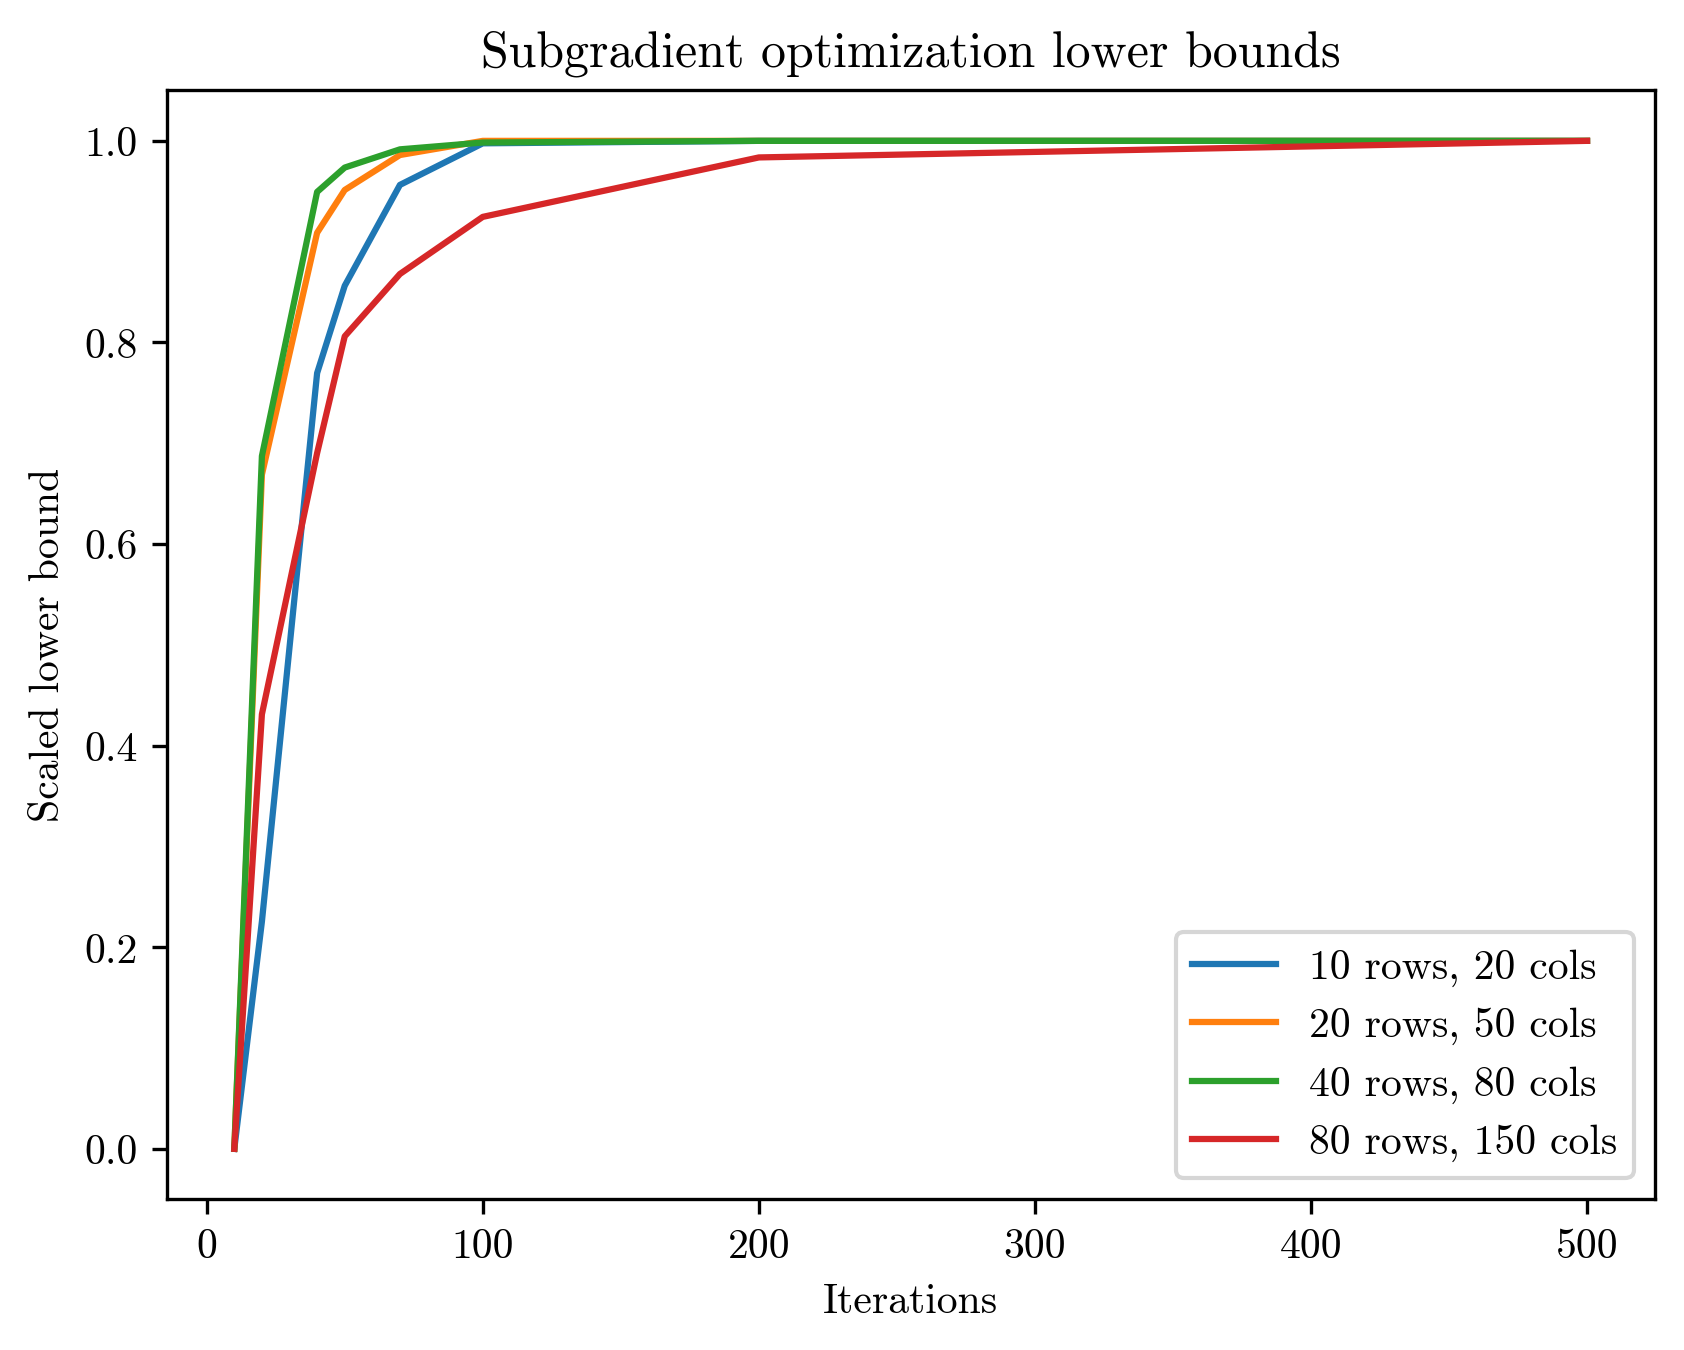
\includegraphics[width=0.7\textwidth]{img/subgrad_lb.png}
  \caption{Sample of images from the USPS dataset. The label is indicated below each image.} 
  \label{fig:dataset:digits}
\end{figure}


\section{Conclusions}
\label{sec:conclusions}

In this work we investigated the performance of the Pegasos algorithm described in Section~\ref{sec:algorithm} on a multiclass classification task over the USPS dataset described in Section~\ref{sec:dataset}. The algorithm was evaluated with 5-fold stratified cross-validation across various settings of hyperparameters. The best performance (0.026 test error with zero-one loss) was achieved by using a polynomial kernel of degree 3, 50000 iterations and a regularization coefficient of 1. A similar performance (0.027 test error) was achieved by using a Gaussian kernel with $\gamma$ equal to 2, 25000 iterations and a regularization coefficient of 1e-5.

The algorithm proved to be an effective classification tool, although the task was not particularly challenging. Moreover, the algorithm showed a noteworthy rate of convergence, bordering a test error of 0.070 after only 1000 iterations when using the Gaussian kernel with $\gamma$ equal to 2.

Further research might explore a wider set of hyperparameters, especially in the direction of lower regularization coefficient values and higher values of $\gamma$ when using a Gaussian kernel.

\bibliographystyle{acm}
\bibliography{bibtex_entries}

\end{document}